\subsection{Neural dynamics}
\label{sec:neural-dynamics}

A common approach to systematically simulate a PING network involves the definition of neural dynamics through the Izhikevich type neuron model  \cite{Izhikevich2003}. This model is plausible enough biologically to mimic genuine neural behavior, yet it is computationally more efficient for large-scale simulations than more biophysically accurate models. The Izhikevich model represents every neuron as dynamical system that can be described with a two-dimensional system of ordinary differential equations (ODEs): for all $v \in V$,
\begin{align}
    \frac{dp_v}{dt} =\ & 0.04 p_v^2 + 5p_v + 140 - r_v + I_v,
    \label{eq:Izhikevich-model-dp-dt} \\
    \frac{dr_v}{dt} =\ & \alpha_{\type(v)} \cdot (\beta_{\type(v)} p_v - r_v), \label{eq:Izhikevich-model-dr-dt} \\
    \text{if } p_v \geq\ & p_{\peak} \text{, then } 
    \begin{cases}
        p_v \leftarrow \gamma_{\type(v)} \\
        r_v \leftarrow r_v + \zeta_{\type(v)}
    \end{cases}, 
    \label{eq:Izhikevich-model-p30}
\end{align}
where
\begin{itemize}
    \item $p_\peak$ is the peak membrane potential ($= 30$ mV);
    
    \item $p$ represents the membrane potential of the neuron; 
    
    \item $r$ represents a membrane recovery variable, which dramatically increases after spikes; it provides negative feedback that suppresses the increase of $p$ and reduces the fluctuations in the output;
    
    \item $\alpha$ describes the timescale of $r$, it is proportional to the recovery speed;
    
    \item $\beta$ describes the sensitivity of $r$ to the subthreshold fluctuations of the membrane potential $p$: greater values of $\beta$ lead to stronger coupling between $p$ and $r$, resulting in more possible subthreshold oscillations;
    
    \item $\gamma$ describes the after-spike reset value of $p$;
    
    \item $\zeta$ describes the after-spike reset value of $r$;
    
    \item $I$ describes the current.
\end{itemize}
It is essential to note that the condition in Equation \ref{eq:Izhikevich-model-p30} involves the peak potential and not the threshold as the latter is dynamic.
The numeric constants in Equation (\ref{eq:Izhikevich-model-dp-dt}) have been obtained by fitting the spike initiation of neural dynamics in such a way that $p$ has a scale of mV, and $t$ - a scale of ms.


The model includes several parameters $\alpha, \beta, \gamma, \zeta$ that control the behavior of the neurons. 
The effects these parameters have on membrane potential and recovery are visualized in Figure \ref{fig:neural-dynamics}. 
The values of $\alpha, \beta, \gamma, \zeta$ correspond to known types of neurons. In this thesis, all excitatory neurons are assumed to be regular spiking (RS) and inhibitory - fast spiking (FS). 
The parameters' values for these types of neurons  are displayed in Table \ref{tab:params-izhikevich-model}.

\begin{figure}[!htp]
    \centering
    % ----- INPUT
\newcommand{\ndimagew}{0.4\textwidth}
\newcommand{\ndimageh}{0.75 * \ndimagew}


\begin{tikzpicture}[
        arr/.style = { -{Stealth[ ]} },
        bluearrow/.style = {arr, draw=third-color, fill=third-color, thick},
        blackarrow/.style = {arr, ultra thick},
    ]
    
    \begin{scope}
    % p(t), r(t)
    \node[] (pt) at (-0.5, 0) {$p(t)$};
    \node[] (rt) at (-0.5, 0.42 * \ndimageh) {$r(t)$};
    
    % peak
    \node[anchor=west] (peaktxt) at (1.1 * \ndimagew, \ndimageh) {\bgcolorsmalltext{third-color}{black}{peak ($30$ mV)}};
    \node[] (peak) at (0.4 * \ndimagew, \ndimageh) {};
    \path [bluearrow] (peaktxt) edge node {} (peak);
    
    % decay alpha 
    \node[anchor=west] (decaytxt) at (1.1 * \ndimagew, 0.2 * \ndimageh) {\bgcolorsmalltext{third-color}{black}{decay with rate $\alpha$}};
    \node[] (decay) at (0.6 * \ndimagew, 0.2 * \ndimageh) {};
    \path [bluearrow] (decaytxt) edge node {} (decay);
    
    % sensitivity beta
    \node[] (senstxt) at (0.6 * \ndimagew, -0.2 * \ndimageh) {\bgcolorsmalltext{third-color}{black}{sensitivity $\beta$}};
    \node[] (sens) at (0.35 * \ndimagew, 0.07 * \ndimageh) {};
    \path [bluearrow] (senstxt) edge node {} (sens);
    
    % reset gamma
    \node[anchor=west] (resetgtxt) at (1.1 * \ndimagew, 0.52 * \ndimageh) {\bgcolorsmalltext{third-color}{black}{reset $\gamma$}};
    \node[] (resetg) at (0.42 * \ndimagew, 0.52 * \ndimageh) {};
    \path [bluearrow] (resetgtxt) edge node {} (resetg);
    
    % reset zeta
    \node[] (resetztxt) at (0.1 * \ndimagew, 0.2 * \ndimageh) {\bgcolorsmalltext{third-color}{black}{reset $\zeta$}};
    \node[] (resetz) at (0.39 * \ndimagew, 0.2 * \ndimageh) {};
    \path [bluearrow] (resetztxt) edge node {} (resetz);
        
    \end{scope}
    
    \begin{scope}
        \node[anchor=south west,inner sep=0] at (0,0) {
\includegraphics[width=\ndimagew]{src/assets/images/neural-dynamics.png}};
    \end{scope}
        
\end{tikzpicture}
    \caption[Effects of Izhikevich parameters on neural dynamics]{Effects of parameters on neural dynamics in the Izhikevich model. {\it This figure is reproduced with permission from \url{www.izhikevich.com}. (Electronic version of the figure and reproduction permissions are freely available at \url{www.izhikevich.com.})}}
    \label{fig:neural-dynamics}
\end{figure}

\begin{figure}[!htp]
    \hspace*{-1.5cm} 
    \centering
    \begin{subfigure}[t]{0.3\textwidth}
        \centering
        % ----- INPUT
\newcommand{\rsimagew}{\textwidth}
\newcommand{\rsimageh}{0.833 * \rsimagew}


\begin{tikzpicture}
    
    \begin{scope}
        \node[] (It) at (-0.5, 0) {$I(t)$};
        \node[] (pt) at (-0.5, 0.22 * \rsimageh) {$p(t)$};
    \end{scope}
    
    \begin{scope}
        \node[anchor=south west,inner sep=0] at (0,0) {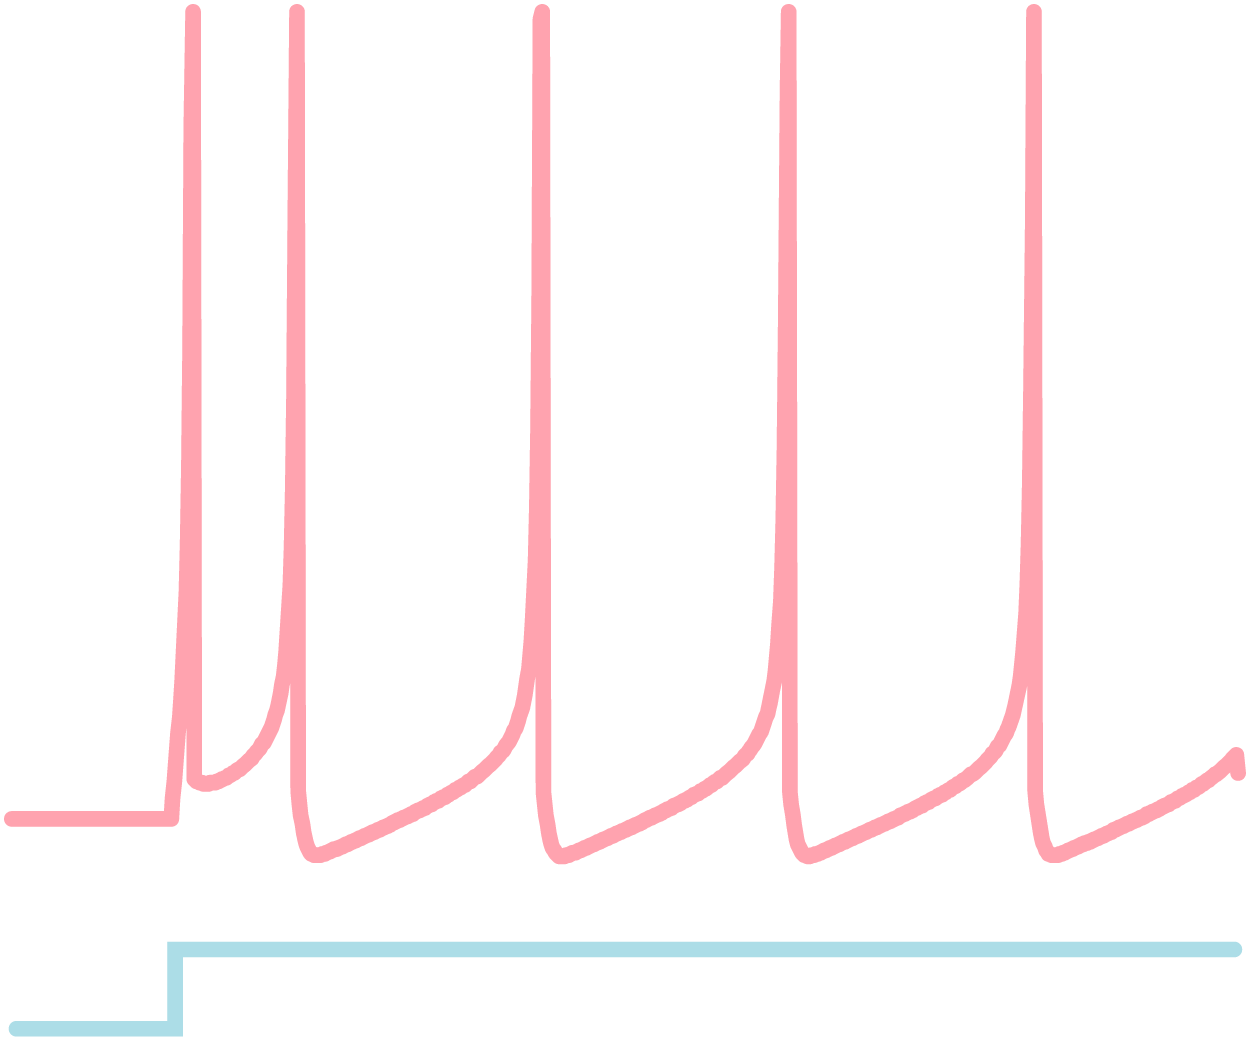
\includegraphics[width=\rsimagew]{src/assets/images/neuron-types/neuron-types_RS.png}};
    \end{scope}
        
\end{tikzpicture}
        \caption{Regular spiking (RS).}
        \label{fig:neuron-types-rs}
    \end{subfigure}
    \hspace{0.1\textwidth}
    \begin{subfigure}[t]{0.3\textwidth}
        \centering
        % ----- INPUT
\newcommand{\fsimagew}{\textwidth}
\newcommand{\fsimageh}{0.833 * \fsimagew}

\begin{tikzpicture}
    
    \begin{scope}
        \node[] (It) at (-0.5, 0) {$I(t)$};
        \node[] (pt) at (-0.5, 0.22 * \fsimageh) {$p(t)$};
    \end{scope}
    
    \begin{scope}
        \node[anchor=south west,inner sep=0] at (0,0) {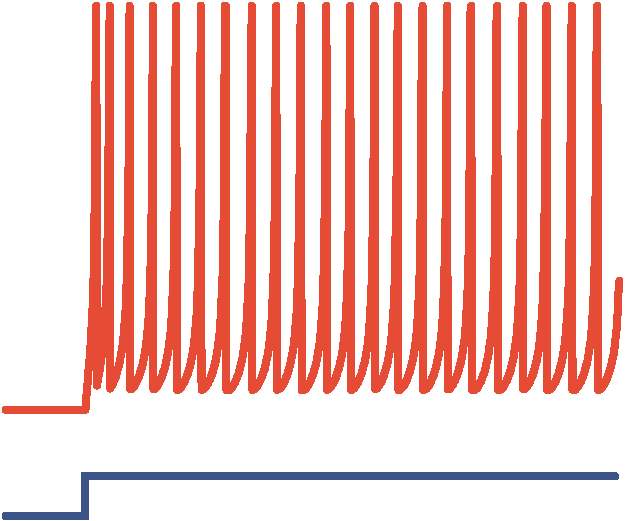
\includegraphics[width=\fsimagew]{src/assets/images/neuron-types/neuron-types_FS.pdf}};
    \end{scope}
        
\end{tikzpicture}
        \caption{Fast spiking (FS).}
        \label{fig:neuron-types-fs}
    \end{subfigure}
    \caption[Spiking behavior of RS and FS neurons]{Spiking behavior of RS and FS neurons in the Izhikevich model. Each horizontal bar represents 20 ms of simulation. {\it This figure is reproduced with permission from \url{www.izhikevich.com}. (Electronic version of the figure and reproduction permissions are freely available at \url{www.izhikevich.com.})}}
    \label{fig:neuron-types}
\end{figure}

\begin{table}[!htp] 
    \centering
    \begin{tabular}{|
    >{\columncolor{main-color}}c |c|c|}
    \hline
    \textbf{Parameter}      & \cellcolor{main-color}\textbf{Excitatory - Regular spiking (RS)} & \cellcolor{main-color}\textbf{Inhibitory - Fast spiking (FS)} \\ \hline
    \textbf{$\pmb{\alpha}$} & 0.02                                                               & 0.1                                                             \\ \hline
    \textbf{$\pmb{\beta}$}  & 0.2                                                                & 0.2                                                             \\ \hline
    \textbf{$\pmb{\gamma}$} & -65                                                                & -65                                                             \\ \hline
    \textbf{$\pmb{\zeta}$}  & 8                                                                  & 2                                                               \\ \hline
\end{tabular}
    \caption[Izhikevich parameters: RS and FS neurons]{Parameters of the Izhikevich model for RS and FS neurons \cite{Izhikevich2003}.}
\label{tab:params-izhikevich-model}
\end{table}


In the present thesis, the network of Izhikevich neurons is simulated by solving the ODEs in Equations (\ref{eq:Izhikevich-model-dp-dt})-(\ref{eq:Izhikevich-model-p30}) using the forward Euler method. The overall simulation time is $\simulationtime = 1000$ ms with the discretization $dt$ of $1$ ms. So, the sequence of time steps $\timesteps \in \mathbb{R}^{\simulationtime \cdot dt}$ is the following:
\begin{equation}
    \timesteps = \left<
        0, 1 \cdot dt, 2 \cdot dt, \cdots, (\simulationtime-1) \cdot dt
    \right>.
\end{equation}

For a neuron $v \in V$, the initial value of the membrane potential is chosen uniformly at random from the range between the resting potential and the peak membrane potential. So, 
\begin{equation}
\begin{gathered}
    p_v(0) \sim U(-65, p_\peak), \\
    r_v(0) = \beta \cdot p_v(0).
\end{gathered}
\end{equation}

\begin{figure}[!htp]
    \centering
    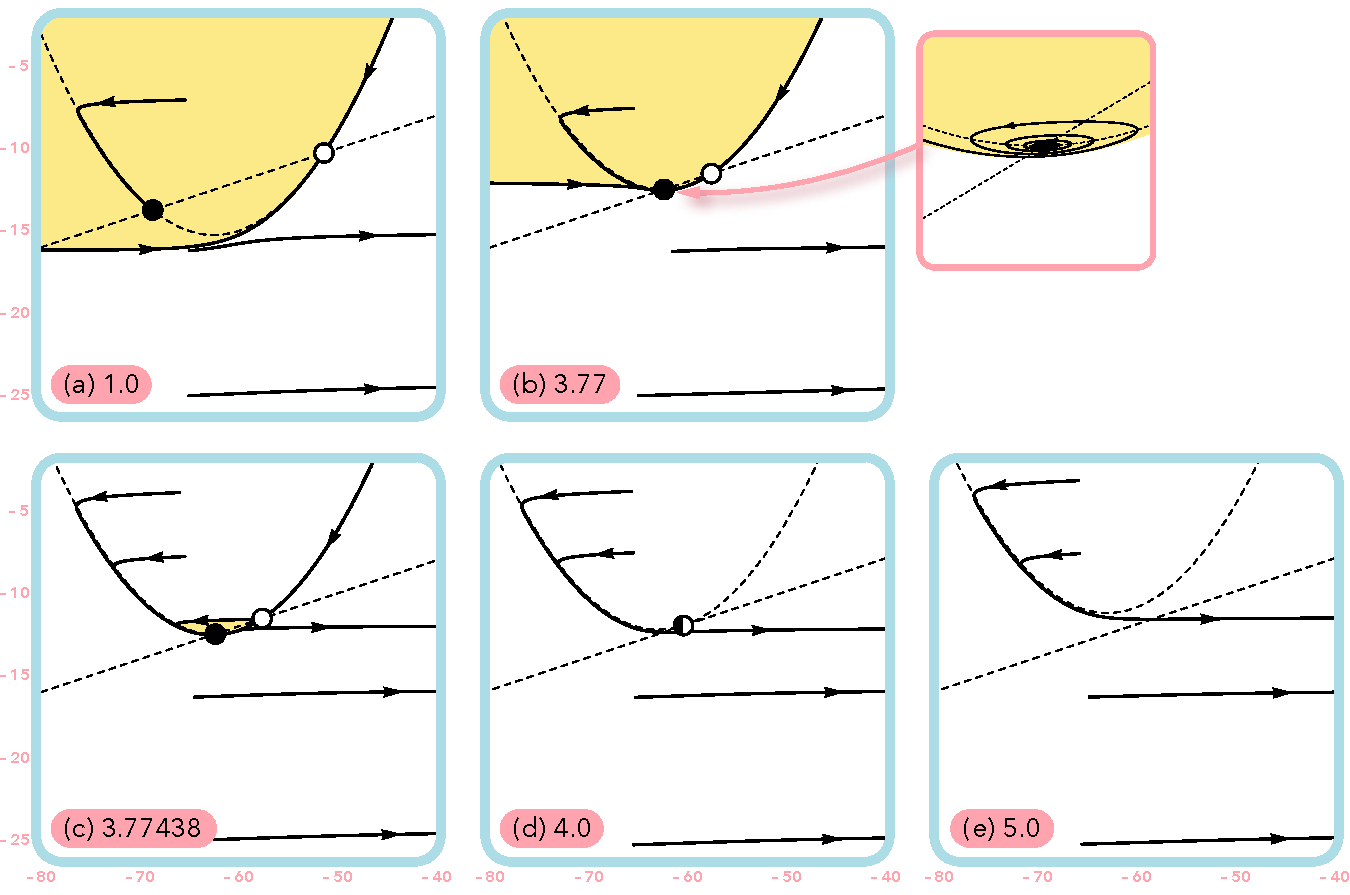
\includegraphics[width=\textwidth]{src/assets/images/neural-dynamics/nd-rs.pdf}
    \caption[Dynamics of an RS neuron]{$p-r$ phase plane: dynamics of an RS neuron depending on current $I_v$.}
    \label{fig:neural-dynamics-rs}
\end{figure}

\begin{figure}[!htp]
    \centering
    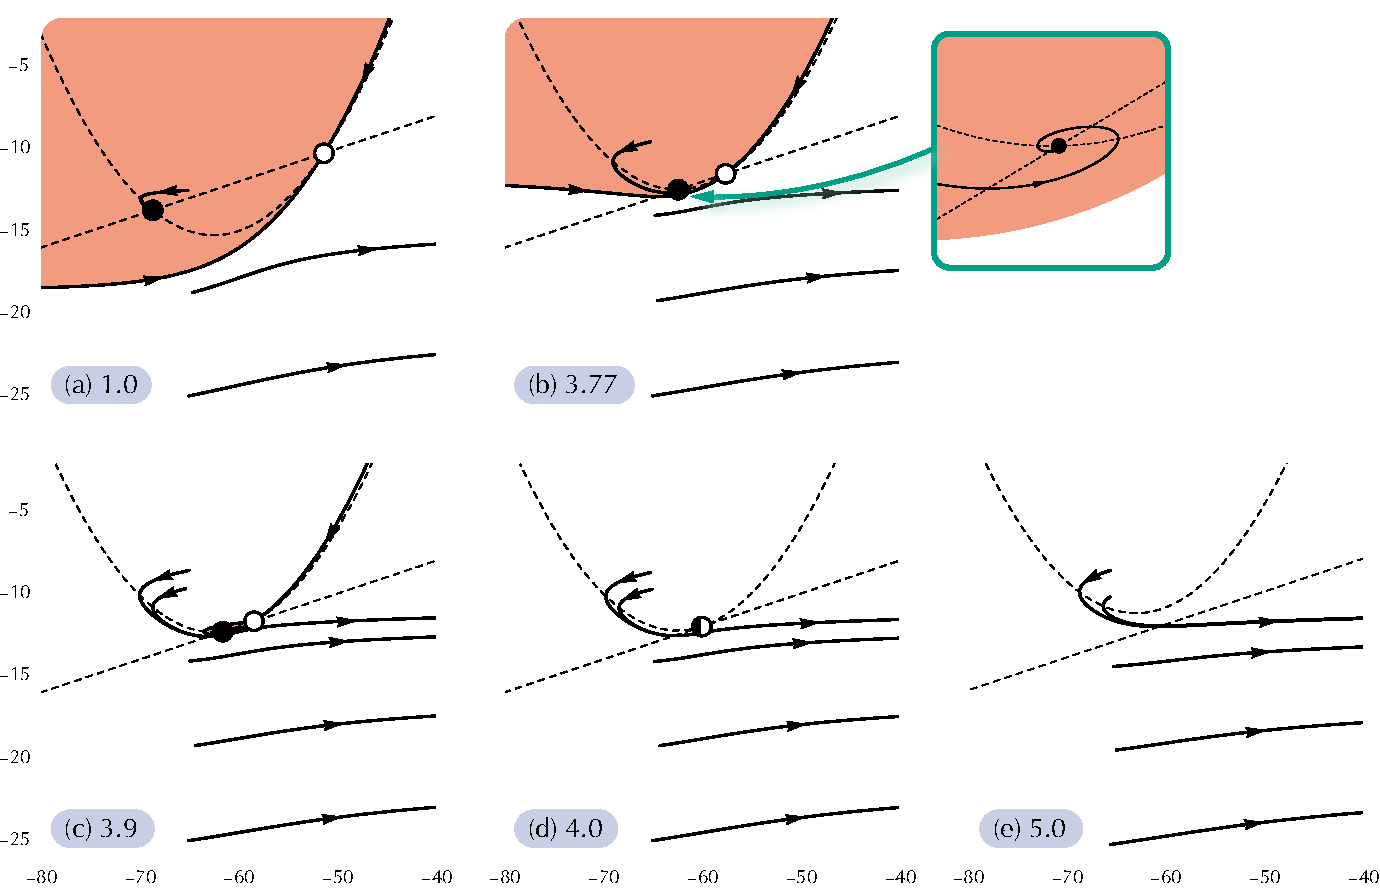
\includegraphics[width=\textwidth]{src/assets/images/neural-dynamics/nd-fs.pdf}
    \caption[Dynamics of an FS neuron]{$p-r$ phase plane: dynamics of an FS neuron depending on current $I_v$.}
    \label{fig:neural-dynamics-fs}
\end{figure}

\paragraph{Regular spiking neurons}

Regular spiking neurons generate spikes with arbitrarily low frequencies that depend on the intensity of applied current, which allows them to encode the input strength \cite{IzhikevichBook2004:10}.
When a stimulus is applied, RS neurons typically first fire with a short interspike period, which later increases (see Figure \ref{fig:neuron-types-rs}). Thus, this neuron type corresponds to the large value of $\zeta$, which causes an after-spike jump in recovery $r$ \cite{Izhikevich2003}.

The spiking dynamics of an RS neuron can be divided into three categories depending on the strength of the input current:
\begin{itemize}
    \item having two stationary points: a node corresponding to the resting state and a saddle,
    \item undergoing a saddle-node bifurcation, where the equilibria annihilate each other, and
    \item having no stationary points.
\end{itemize}

When a small depolarizing current, such as in Figure \ref{fig:neural-dynamics-rs}a, is applied, the nullclines (dashed lines) on the $p-r$ phase plane intersect twice, resulting in two stationary points: a stable node $\circletfill$ corresponding to the resting state and a saddle $\circlet$. The attraction basin on the former (the shaded area) is bounded by the stable manifold of the latter. When the initial pair of values, $p_v$ and $r_v$, lies outside the basin, the neuron produces a finite number of spikes. The recovery value resets closer to the stable manifold with each spike and eventually emerges in the attraction basin. Then, the neuron undergoes hyperpolarization before returning to its resting state. As the current grows, the attraction domain of the stable node shrinks, as illustrated in Figure \ref{fig:neural-dynamics-rs}b, and the trajectories starting there lead to dumped subthreshold oscillations. With further increase of the current, the basin closes and forms a homoclinic orbit (that originates and terminates at the saddle), as shown in Figure \ref{fig:neural-dynamics-rs}c. The event prompts the appearance of the limit cycle attractor. All trajectories starting outside the orbit converge to the limit cycle, where they fire indefinitely. As the current increases further, the system undergoes a saddle-node bifurcation: the homoclinic orbit collapses on itself, and the equilibria annihilate each other, labeled as $\circletfillhl$ in Figure \ref{fig:neural-dynamics-rs}d. Currents causing the mentioned bifurcation and larger lead to unconditional infinite firing (Figure \ref{fig:neural-dynamics-rs}e) as no stationary points exist.


\paragraph{Fast spiking neurons}

Similar to RS neurons, the frequency of FS neurons varies depending on the intensity of the applied current. Additionally, the phase portrait and dynamical behavior of FS neurons are qualitatively similar to those of RS neurons (Figure \ref{fig:neural-dynamics-fs}). Although, in contrast to the latter, FS neurons have a smaller after-spike reset value of the recovery variable ($\zeta$), which, in combination with a faster recovery rate ($\alpha$), allows for spikes with higher frequency (see Figure \ref{fig:neuron-types-fs}) and damped oscillations with higher friction.